\documentclass[10pt]{article}
\nonstopmode
\usepackage{multicol}
\usepackage{times}
\usepackage{tikz}
\usetikzlibrary{positioning}
\usetikzlibrary{calc}
\usetikzlibrary{chains}
\usetikzlibrary{shapes.misc}
\usetikzlibrary{shapes.symbols}
\usetikzlibrary{shapes.geometric}
\usetikzlibrary{fit}
\usetikzlibrary{shadows}
\usepackage{sectsty}
\usepackage[utf8]{inputenc}
\allsectionsfont{\sffamily}
\usepackage{microtype}
\usepackage{graphicx}
\usepackage{verbatim}
\usepackage{lipsum}
\parskip=0.5em

\usepackage[a4paper,margin=2cm]{geometry}

\pagestyle{empty}
\parindent=0cm

\begin{document}%
%
\begin{tikzpicture}[remember picture,overlay,opacity=0.2]
  \node [below=3cm of current page.north] {
    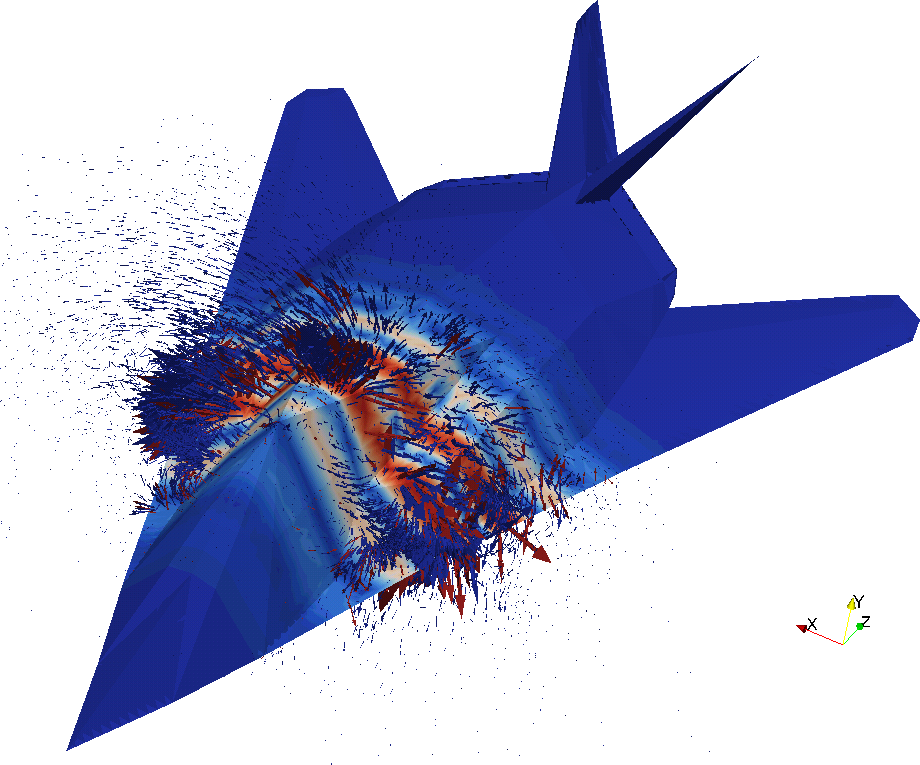
\includegraphics[width=1.2\textwidth]{f117-arrows.png}
  } ;
\end{tikzpicture}
\vspace{-5ex}

\begin{center}
  \fontfamily{phv}
  {\bfseries\Large
    Computer code too slow?\\[2mm]
  }
  {\bfseries\huge
    Learn \emph{High-Performance Computing}

    at NYU this fall!
  }

\end{center}

\begin{multicols}{2}
\Large

{\sffamily\Large\bfseries What will you learn in this class?}

You will learn how to write programs that run fast and use computers
efficiently.

If you have a computation-heavy problem that you would like to go
faster, you're especially welcome.

\begin{comment}
\textbf{Pop Quiz:} \$400 at your favorite electronics retailer
buys you a parallel computer that will do
$4\cdot 10^{12}$ floating point operations (``flops'') per second,
but only load $5\cdot 10^{10}$ values from memory in the same
amount of time. How do you use such a machine well?
\end{comment}

\vspace{2.5ex}
{\sffamily\Large\bfseries What to expect}
\vspace{-1.5ex}
\begin{itemize}
\setlength{\itemsep}{-1mm}
  \item Basic processor architecture
    Performance of sequential code
  %\item Why go parallel? Forms of parallelism
  \item Shared Memory and \textbf{OpenMP}
  \item Distributed Memory and \textbf{MPI}
  \item \textbf{GPUs} and \textbf{OpenCL}
  \item Tools and Debuggers
  \item Examples drawn from numerical linear algebra and numerical
    methods for PDEs
  %\item Common Patterns in Parallel Algorithms
\end{itemize}

Class and homework assignments will be based on C.
(warm-up provided for those coming from
Java or Fortran)

\emph{Assessment:} Weekly homework, final
project. (recommended even if auditing)

We're looking forward to seeing you in the fall!
\vspace{1.5ex}

\hfill
\begin{minipage}{0.4\columnwidth}
  \raggedright
  \emph{Marsha Berger}
  \small\texttt{berger@cims.nyu.edu}
\end{minipage}
\hfill
\begin{minipage}{0.5\columnwidth}
  \raggedright
  \emph{Andreas Klöckner}
  \small \texttt{kloeckner@cims.nyu.edu}
\end{minipage}

%\centering
%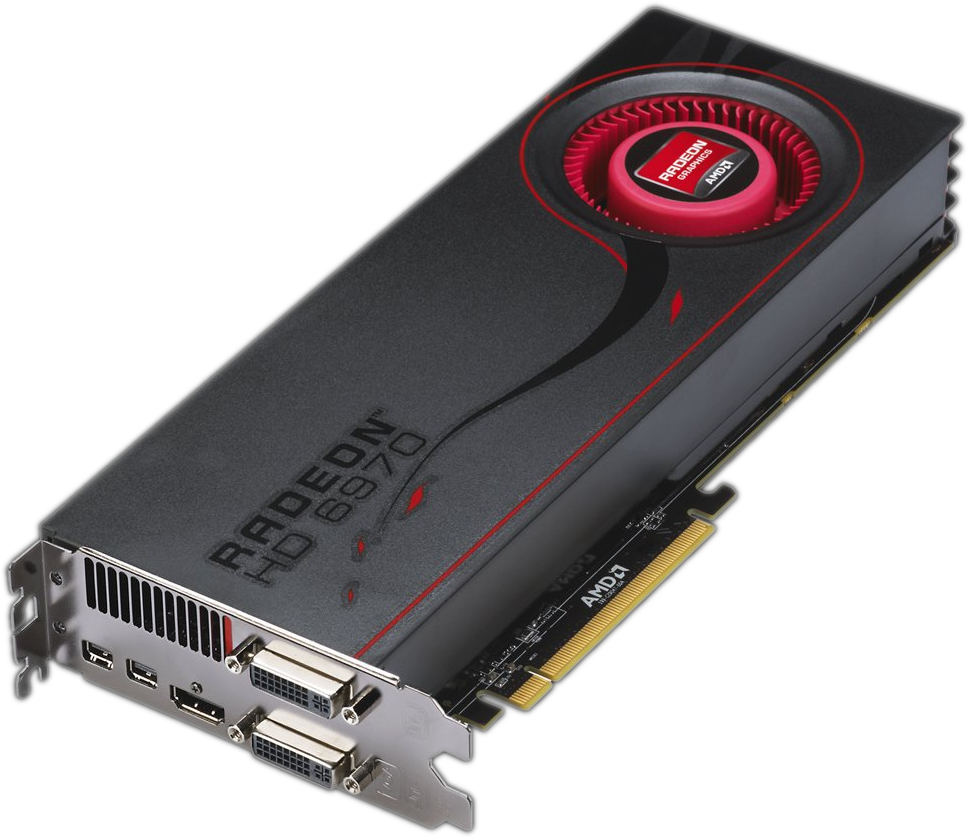
\includegraphics[width=0.6\columnwidth]{amd-6970.png}

\end{multicols}

\begin{center}
  \fontfamily{phv}
  {\bfseries\LARGE
    Save the date! (Room TBD) http://bit.ly/hpc12\\[1em]

    \Huge
    Fall Semester 2012, Wednesdays 5-7pm
  }
\end{center}

\begin{center}
  \begin{minipage}{0.2\textwidth}
    \centering
    
\includegraphics[width=0.8\textwidth]{hpc-qr.png}

    \LARGE\textsf{bit.ly/hpc12}
  \end{minipage}%
  \begin{minipage}{0.2\textwidth}
    \centering
    
\includegraphics[width=\textwidth]{opencl-logo.png}

    \Large\fontfamily{phv}\selectfont OpenCL
  \end{minipage}%
  \begin{minipage}{0.2\textwidth}
    \centering
    
\includegraphics[width=0.8\textwidth]{openmpi-logo.pdf}

    \Large\fontfamily{phv}\selectfont MPI
  \end{minipage}%
  \begin{minipage}{0.2\textwidth}
    
\includegraphics[angle=35,width=\textwidth]{openmp-logo.png}
  \end{minipage}%
  \begin{minipage}{0.2\textwidth}
    \centering
    
\includegraphics[width=0.7\textwidth]{nyu-logo.pdf}
  \end{minipage}
\end{center}

\begin{tikzpicture}[remember picture,overlay]
  \foreach\i in {0,...,9}
  {
    \path (current page.south west) ++(\i*2.1,0) coordinate (tearbase\i) ;
    \node [anchor=north west,rotate=90,xshift=2em,yshift=-2em] at (tearbase\i) 
    { \fontfamily{phv}\huge bit.ly/hpc12 } ;
    \draw (tearbase\i) -- ++(0,5cm) ;
  }
\end{tikzpicture}
%\begin{minipage}{0.45\textwidth}
%\begin{center}
\end{document}

